\section{问题总览：长程智能体为什么需要新记忆形态}

本章的结论很直接：长程智能体的记忆瓶颈来自统一的 token 密度。文本记忆会把关键证据、supporting facts 和琐碎 details 都放进同一种线性 token 流里；一旦 memory budget 收紧，系统缺少一种天然机制来优先保护真正影响 final answer 的信息。MemOCR 的出发点正是把记忆从一维文本串推向二维视觉画布，让信息的重要性通过版面显著性和压缩强度表现出来。

\begin{importantbox}{本章核心判断}
长程推理中的关键问题集中在“变短时谁先被保留下来”。若所有信息都以同等 token 密度存在，100 个 token 的关键证据可能需要携带约 900 个 token 的辅助事实与细节，最终让真正有用的信息被预算压力一起拖下水。
\end{importantbox}

\subsection{长程推理的真实瓶颈：历史持续增长}

讲者介绍的主题是 \textit{MemOCR: Layout-Aware Visual Memory for Efficient Long-Horizon Reasoning}。其中 \textit{long-horizon reasoning} 指智能体跨越大量步骤、长时间窗口或多轮交互完成任务的能力。代码智能体、LongCat 这类 long-horizon task 都属于典型场景：任务执行过程越长，历史交互越多，模型越需要保存中间判断、外部观察、失败尝试、用户偏好和可复用证据。

\textit{Agentic memory} 可以理解为智能体的工作笔记系统。一个人写长篇技术报告时，会把资料、待办、引用、草稿和判断依据放进笔记；智能体也需要类似机制，把历史交互保存、压缩、检索并重新用于后续决策。问题在于，模型的上下文窗口始终有限，推理阶段真正能塞进 prompt 的内容更有限。历史长度增长通常近似线性：

$$
|H_t| = \sum_{i=1}^{t} |h_i|
$$

这里的符号含义如下：

\begin{itemize}
  \item $H_t$：截至第 $t$ 步积累下来的历史交互集合。
  \item $h_i$：第 $i$ 步产生的一段交互、观察或中间结果。
  \item $|h_i|$：该片段占用的 token、字符或等价上下文容量。
\end{itemize}

当 $t$ 持续增大时，完整历史很快超过可用 context budget。此时智能体必须做压缩，压缩策略的质量会直接决定后续推理是否还能找到关键证据。

\begin{knowledgebox}{memory budget 与 context budget}
\textit{Context budget} 是模型一次推理能接收的总上下文容量，包括问题、系统指令、工具返回、历史摘要和其他输入。\textit{Memory budget} 是其中专门分配给记忆表示的预算，在本讲中常指最终回答阶段用于表示视觉记忆的 image tokens。前者像整张书桌，后者像书桌上留给笔记本的一块区域；笔记本再重要，也无法占满整张书桌。
\end{knowledgebox}

\subsection{两类传统记忆：原始历史与文本摘要}

讲者把既有 agentic memory 方法概括为两类。第一类是 \textit{raw history memory}，即保留原始历史，把大量交互放进一个 corpus，再通过 top-$k$ retrieval 找回相关片段。这类方法的优点是原始证据损失少，风险是检索和上下文成本高；它像把全部资料都装进档案柜，查找时再抽取可能相关的文件。

第二类是 \textit{textual summary memory}，即让智能体主动把历史压缩成文本摘要。它能把很长的交互压成较短的 memory state，例如讲者用约 \(1K\) token 表示压缩后的文本记忆长度。它像把整场会议整理成一页纪要，读取成本比原始档案低很多。

这两类方法的差异很明显：raw history memory 更接近“保真”，textual summary memory 更接近“概括”。两者共同面对同一个硬约束：最终进入模型的内容仍然以线性 token 串表达。只要进入线性文本，重要事实和辅助细节就会被同一种计价单位衡量。

\begin{figure}[H]
\centering
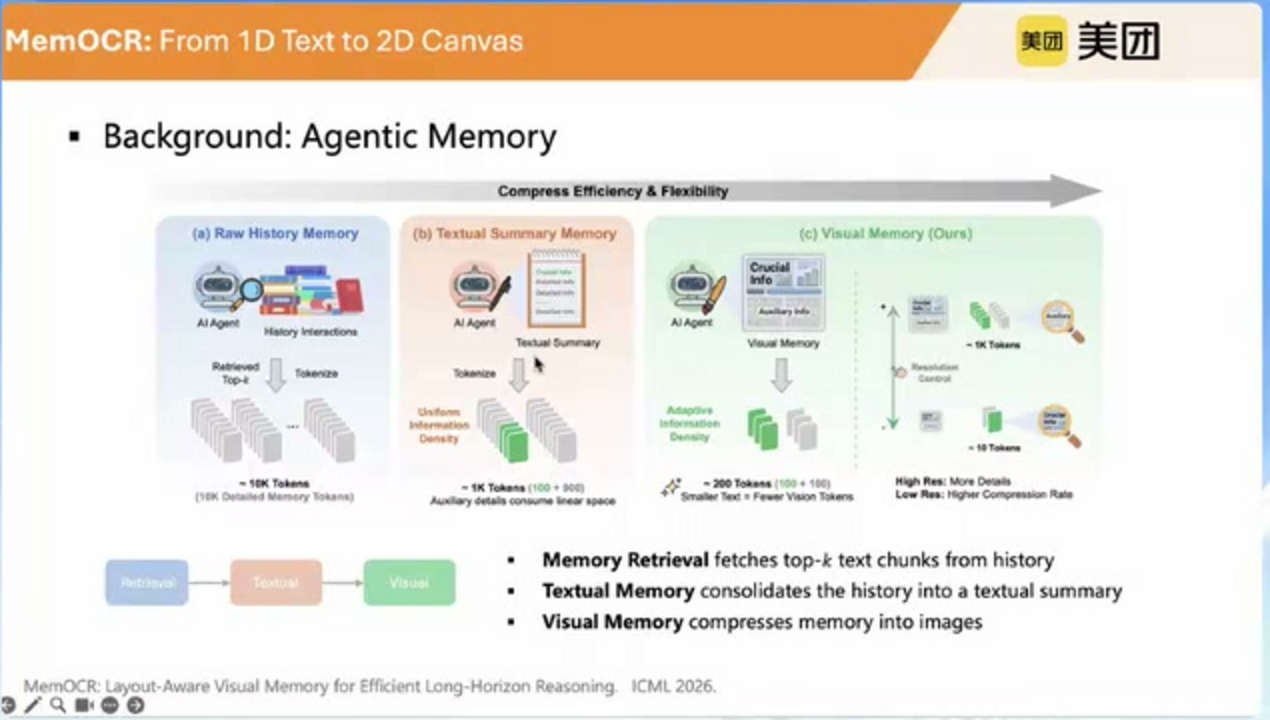
\includegraphics[width=0.82\linewidth,height=0.36\textheight,keepaspectratio]{figures/selected/fig01_agentic_memory_background.png}
\caption{Agentic memory 的三类形态：raw history memory 依赖检索，textual summary memory 依赖线性摘要，visual memory 用二维布局表达信息密度与压缩强度。\protect\footnotemark}
\label{fig:agentic-memory-background}
\end{figure}
\footnotetext{视频画面时间区间：00:02:30--00:03:00。}

图~\ref{fig:agentic-memory-background} 的关键读法是看中间与右侧的差异。textual summary memory 中所有内容进入同一条 token 流；visual memory 中，关键信息可以占据更醒目的视觉区域，辅助信息可以进入较低显著性的区域，整体还可以通过分辨率调整实现全局压缩。

\subsection{统一 token 密度为什么浪费预算}

文本摘要的深层问题是统一信息密度。无论某句话是直接决定答案的关键证据，还是只帮助读者理解背景的 supporting fact，它们在 token 层面都占用同样性质的预算。文本串缺少“这一块更醒目、那一块更细小”的自然表达。

可以用一个简化预算式来理解：

$$
C_{\text{text}} = C_{\text{key}} + C_{\text{support}} + C_{\text{detail}}
$$

这里的符号含义如下：

\begin{itemize}
  \item $C_{\text{text}}$：文本记忆总预算。
  \item $C_{\text{key}}$：关键证据占用的预算。
  \item $C_{\text{support}}$：支撑事实占用的预算。
  \item $C_{\text{detail}}$：细节、背景和解释性信息占用的预算。
\end{itemize}

若关键证据约为 \(100\) tokens，supporting facts 与 details 合计约为 \(900\) tokens，则关键证据比例为：

$$
r_{\text{key}} = \frac{100}{100 + 900} = 0.1
$$

这表示真正决定答案的信息只占约 \(10\%\) 的文本预算。预算被压缩时，系统如果只按长度删减，很容易同时削弱关键证据和辅助材料。直觉上，这像把证件、衣物和备用物品都塞进同一个旅行箱，并且没有单独的证件袋；容量一紧，系统知道“箱子太满”，却缺少可靠信号判断哪一件东西应该最先保护。

\begin{warningbox}{容易误解的地方}
文本摘要变短并不自动意味着记忆更有效。有效记忆需要同时回答四个问题：存什么、压多狠、放在哪里、读得出来吗。只回答“压缩到多短”会漏掉证据优先级和读取可行性这两个关键约束。
\end{warningbox}

MemOCR 引入视觉记忆的第一性原理可以概括为：信息价值不同，压缩强度也应不同。视觉画布提供了文本串缺少的表达自由度：字号、位置、标题层级、留白、分区和显著性都能传递优先级。关键证据可以像白板上的大标题，辅助事实可以像边栏小字；在下采样或 image token 预算变小时，大标题仍更可能被保留下来。

\subsection{本章小结}

本章建立了 MemOCR 的问题背景。长程智能体需要记住越来越多的历史，raw history memory 保真度高但代价大，textual summary memory 更紧凑却仍受线性 token 密度限制。统一 token 密度会让关键证据与辅助细节共享同一预算压力，导致 memory budget 紧张时真正影响答案的信息缺少优先保护机制。下一章将沿着这个矛盾进入 MemOCR 的核心转向：把记忆从 text domain 搬到 vision domain，用二维布局承载信息优先级。
